\documentclass{article}
\usepackage[utf8]{inputenc}
\usepackage{amsmath}
\usepackage{amssymb}
\usepackage{amsthm}
\usepackage{enumerate}
\usepackage{mathtools}
\usepackage{float} % For plassering av bilder
\usepackage{a4wide} % mer width
\usepackage{amsmath}
\usepackage{amssymb}
\usepackage{parskip}

\usepackage[colorlinks=false,allcolors=blue]{hyperref}
%Fikser hyperref
\addto\extrasnorsk{%
\def\figureautorefname{Figure}%
\def\tableautorefname{Table}%
\def\sectionautorefname{section}%
\def\subsectionautorefname{subsection}%
}
% Vi endrer fonten som brukes for URLer til den vanlige tekstfonten.
\urlstyle{same}


% FRA IC
\usepackage{natbib}
\usepackage{amsmath}
\usepackage{listings}
\usepackage{graphicx}
\usepackage[inline]{enumitem}
\usepackage{xcolor}
 \usepackage{booktabs}
\date{}
\newcommand*{\boxednumber}[1]{%
    \expandafter\readdigit\the\numexpr#1\relax\relax
}
\newcommand*{\readdigit}[1]{%
    \ifx\relax#1\else
        \boxeddigit{#1}%
        \expandafter\readdigit
    \fi
}
% Format macro used for every digit, adjust to your liking:
\newcommand*{\boxeddigit}[1]{\fbox{#1}\hspace{-\fboxrule}}

\usepackage[left=4cm,right=4cm,vmargin=1.5cm,footnotesep=0.5cm]{geometry}
\setlength\parindent{0pt}



\title{TDT4265 - Computer Vision and Deep Learning \\Assignment 2}
\author{Jakob Vahlin & Kristian Stensgård}
%\date{September 2020}

\begin{document}

\maketitle

\tableofcontents
\newpage

\section{Softmax regression with backpropagation}
\subsection{Task 1a: Backpropagation}

\subsubsection*{i)}
\textit{Notation:} To easier distinguish between $z$ values when deriving certain calculations, $z^o$ will mean KANSKJE?????



In the neural network considered in this assignment the gradient descent update rule for weights $w_{ji}$ of the \textbf{hidden} layer is given by

\begin{equation}
    w_{j i}:=w_{j i}-\alpha \frac{\partial C}{\partial w_{j i}} , \quad \alpha \in \mathbb{R}
    \label{eq:1a_start}
\end{equation}
where $C(w)$ is the cross entropy loss, defined by
\begin{equation}
    C(w)=\frac{1}{N} \sum_{n=1}^{N} C^{n}(w), \quad C^{n}(w)=-\sum_{k=1}^{K} y_{k}^{n} \ln \left(\hat{y}_{k}^{n}\right)
    \label{eq:cross_entropy}
\end{equation}
where $\hat{y}$ is the Softmax activation function for the \textit{output} layer, defined by

\begin{equation}
    \hat{y}_{k}=\frac{e^{z_{k}}}{\sum_{k^{\prime}}^{K} e^{z_{k^{\prime}}}}, \quad \text { where } z_{k}=w_{k}^{T} \cdot a=\sum_{j}^{J} w_{kj} \cdot a_{j}
    \label{eq:softmax}
\end{equation}

where $w_{kj}$ are weights in the output layer and $a_j = f(z_j)$ is the is the Sigmoid activation function for a node (neuron?) in the \textit{hidden} layer, defined as

\begin{equation}
    a_j =  f(z_j)=\frac{1}{1+e^{-z_j}}, \quad z_j = w_j^{T} x=\sum_{i}^{I} w_{ji} \cdot x_{i}
    \label{eq:sigmoid}
\end{equation}



By algebraic manipulation it can be shown that \eqref{eq:1a_start} can be written as

\begin{equation}
    w_{j i}:=w_{j i}-\alpha \delta_{j} x_{i}
    \label{eq:1a_goal}
\end{equation}

by defining $\delta_{j}=\frac{\partial C}{\partial z_{j}}$.

To derive the equvialent expression for the gradient descent update rule given by \eqref{eq:1a_goal} consider the partial derivative of the cross entropy loss function w.r.t the variable $w_{ji}$. From \eqref{eq:cross_entropy} and \eqref{eq:softmax} it is clear that $C(w)$ has a dependence on $z_k$. Furthermore, from \eqref{eq:softmax}, it is clear that $z_k$ in turn has a dependence on $a_j$, which in turn has a dependence on $z_j$, as evident from \eqref{eq:sigmoid}. Finally, from \eqref{eq:sigmoid} it is clear that $z_j$ has a dependence on $w_{ji}$. Consequently, the cost functions dependence on the variable $w_{ji}$ is ``chained together'' through the variables $z_k$,$a_j$ and $z_j$. By defining $\boldsymbol{z_{o}} = [z_1,z_2,\dots,z_K]$ as the vector containing $z$ values from the output layer, $\boldsymbol{a} = [a_1,a_2,\dots,a_J]$ as the vector with $a$ values from the hidden layer and $\boldsymbol{z_h} = [z_1,z_2,\dots,z_J]$ as the vector containing $z$ values from the hidden layer, we can express the cross entropy loss function in terms of its variables in the following way
\begin{align}
\begin{split}
    C(w) &= C(\boldsymbol{z_o}) \\ 
    &= C\big(\boldsymbol{z_o}(\boldsymbol{a})\big) \\
    &= C\bigg(\boldsymbol{z_o}\big(\boldsymbol{a}(\boldsymbol{z_h})\big)\bigg) \\
    &= C\bigg(\boldsymbol{z_o}\big(\boldsymbol{a}(\boldsymbol{z_h}(w))\big)\bigg)
    \label{eq:cost_var_def}
\end{split}
\end{align}

with $K$ representing the number of nodes in the output layer, and $J$ representing the number of nodes in the hidden layer. In this case, the lowercase $w$ represents the weight matrix from the input layer to the hidden layer, in accordance with the notation in the assignment description (later in the report matrices will be represented by bold, uppercase letters). Therefore, the derivative of the cross entropy loss function, w.r.t to any weight in the \textit{hidden} layer $w_{ji}$, $\frac{\partial C}{\partial w_{ji}}$, can be expressed by applying the multivariate chain rule.

In the following, to distinguish between $z$ vector from the different layers in the network, entries from the $z$ vector from the hidden layer will be labeled $z^j$ and entries from the $z$ vector from the output layer will be labeled $z^k$. This is needed to distinguish between i.e $z_{1}$ from the hidden layer and $z_1$ from the output layer.

\begin{align}
\begin{split}
    \frac{\partial C}{\partial w_{ji}} &= \frac{\partial C}{\partial z_1^k} \Bigg( 
    \frac{\partial z_1^k}{\partial a_1}\frac{\partial a_1}{\partial  z^j_1} \frac{\partial z^j_1}{\partial w_{1i}} + \frac{\partial z_1^k}{\partial a_2}\frac{\partial a_2}{\partial  z^j_2} \frac{\partial z^j_2}{\partial w_{2i}} + \dots + \frac{\partial z_1^k}{\partial a_J}\frac{\partial a_J}{\partial  z^j_J} \frac{\partial z^j_J}{\partial w_{Ji}}\Bigg) \\
    &+ \frac{\partial C}{\partial z_2^k} \Bigg( 
    \frac{\partial z_2^k}{\partial a_1}\frac{\partial a_1}{\partial  z^j_1} \frac{\partial z^j_1}{\partial w_{1i}} + \frac{\partial z_2^k}{\partial a_2}\frac{\partial a_2}{\partial  z^j_2} \frac{\partial z^j_2}{\partial w_{2i}} + \dots + \frac{\partial z_2^k}{\partial a_J}\frac{\partial a_J}{\partial  z^j_J} \frac{\partial z^j_J}{\partial w_{Ji}}\Bigg) \\
    &+ \dots + \frac{\partial C}{\partial z_K^k} \Bigg( 
    \frac{\partial z_K^k}{\partial a_1}\frac{\partial a_1}{\partial  z^j_1} \frac{\partial z^j_1}{\partial w_{1i}} + \frac{\partial z_1^k}{\partial a_2}\frac{\partial a_2}{\partial  z^j_2} \frac{\partial z^j_2}{\partial w_{2i}} + \dots + \frac{\partial z_1^k}{\partial a_J}\frac{\partial a_J}{\partial  z^j_J} \frac{\partial z^j_J}{\partial w_{Ji}}\Bigg) 
\end{split} \label{eq:chain}
\end{align}

Equation \eqref{eq:chain} can be simplified to a set of sums (\textit{Notation}: Note that as there no longer exist a need to distinguish between $z$ vectors from the different layers in the network, as this will now be clear from the variable ($j$ or $k$) used to index the vectors in accordance with the notation in the assignment description).   

\begin{equation}
    \frac{\partial C}{\partial w_{ji}} = \sum_{k=1}^K \frac{\partial C}{\partial z_k}\Bigg( \sum_{j'=1}^J \frac{\partial z_k}{\partial a_{j'}}\frac{\partial a_{j'}}{\partial z_{j'}}\frac{\partial z_{j'}}{\partial w_{ji}} \Bigg)
    \label{eq:chain_sum}
\end{equation}

To further simplify \eqref{eq:chain_sum}, consider the last partial derviative, $\frac{\partial z_{j'}}{\pratial w_{ji}}$. From the definition of $z_j$ given in \eqref{eq:sigmoid} the derivative w.r.t to $w_{ji}$ can be expressed as

\begin{equation}
    \frac{\partial z_{j'}}{\partial w_{ji}} = \frac{\partial}{\partial w_{ji}} \sum_{i'=1}^I w_{j'i'}x_{i'}, \quad \text{for a given \textit{j'}}
    \label{eq:diffzj}
\end{equation}

Similar to when deriving the gradients of the cost function in Assignment 1, the resulting differentiation of the sums in \eqref{eq:diffzj} w.r.t to a given given weight, $w_{j'i'}$ will only be non-zero for $j' = j$ and $i' = i$. When this is the case the differentiation of $z_{j'} = z_j$ becomes

\begin{align}
\begin{split}
    \frac{\partial z_{j}}{\partial w_{ji}} &= \frac{\partial }{\partial w_{ji}} \sum_{i'=1}^I w_{ji'}x_{i'} \\
    &= \frac{\partial}{\partial w_{ji}} w_{ji}x_i \\
    &= x_i
\end{split}
\label{eq:diffzjdone}
\end{align}
 
 Thus it is clear that $\frac{\partial z_{j'}}{\partial w_{ji}} = x_i$, for $j' = j$ and thus it is independent of the $j'$ and $k$ indecies. Consequently it can be moved outside of the sums that goes over all $j'$ and over all $k$.
 
\begin{align}
\begin{split}
    \frac{\partial C}{\partial w_{ji}} &= \sum_{k=1}^K \frac{\partial C}{\partial z_k}\Bigg( \sum_{j'=1}^J \frac{\partial z_k}{\partial a_{j'}}\frac{\partial a_{j'}}{\partial z_{j'}}\frac{\partial z_{j'}}{\partial w_{ji}} \Bigg) \\
    &=  \sum_{k=1}^K \frac{\partial C}{\partial z_k}\Bigg( \sum_{j'=1}^J \frac{\partial z_k}{\partial a_{j'}}\frac{\partial a_{j'}}{\partial z_{j'}}x_i \Bigg) \\
    &=  \Bigg(\sum_{k=1}^K \frac{\partial C}{\partial z_k}\Bigg( \sum_{j'=1}^J \frac{\partial z_k}{\partial a_{j'}}\frac{\partial a_{j'}}{\partial z_{j'}}\Bigg)\Bigg) x_i
    \label{eq:movexiout}
\end{split}
\end{align}

KAN STRENGT TATT LA VÆRE Å BRUKE J' INDEKS HERIFRA OG UT, MEN VURDER Å LEGGE TIL LIKVEL / FORKARE HVORFOR.

Furthermore, consider the definition of $\delta_j$, given by

\begin{equation}
    \delta_j = \frac{\partial C}{\partial z_j}
    \label{eq:deltadef}
\end{equation}
 
 From the chain of dependencies given in \eqref{eq:cost_var_def}, the derivative in \eqref{eq:deltadef} can be expressed by applying the multivariate chain rule
 
\begin{equation}
    \delta_j = \frac{\partial C}{\partial z_j} = \sum_{k=1}^K \frac{\partial C}{\partial z_k} \bigg(\sum_{j=1}^J\frac{\partial z_k}{\partial a_j}\frac{\partial a_j}{\partial z_j} \bigg)
    \label{eq:djchain}
\end{equation}
By inserting the result in \eqref{eq:djchain} into \eqref{eq:movexiout}, the derivative of the cost function w.r.t $w_{ji}$ becomes

\begin{align}
\begin{split}
     \frac{\partial C}{\partial w_{ji}} &= \Bigg(\sum_{k=1}^K \frac{\partial C}{\partial z_k}\Bigg( \sum_{j=1}^J \frac{\partial z_k}{\partial a_j}\frac{\partial a_j}{\partial z_j}\Bigg)\Bigg) x_i \\
     &= \frac{\partial C}{\partial z_j} x_i \\
     &= \delta_j x_i
\end{split}
\label{eq:dif_done}
\end{align}

Finally, inserting the result in \eqref{eq:dif_done} into \eqref{eq:1a_start}, the desired result given by \eqref{eq:1a_goal} is found. \qed

\subsubsection*{ii)}

With $\delta_j$ defined as

\begin{equation}
\delta_j = \frac{\partial C}{\partial z_j}
    \label{eq:deltaj}
\end{equation}
where $z_j$ is defined as in \eqref{eq:softmax}, it can be shown that $\delta_j$ can be expressed as

\begin{equation}
    \delta_j = f'(z_j)  \sum_{k=1}^K w_{kj} \delta_k
    \label{eq:part2goal}
\end{equation}
where $\delta_k = \frac{\partial C}{\partial z_k} = -(y_k - \hat{y}_k)$ and $f'(z_j) = \frac{\partial f}{\partial z_j} = \frac{\partial a_j}{\partial z_j}$ is the slope of the Sigmoid activation function for the hidden layer, given by \eqref{eq:softmax}.

To prove the relationship given by \eqref{eq:part2goal}, recall from part \textit{i)} and \eqref{eq:djchain} the definition of $\delta_j$ with the derivative written out according to the chain rule

\begin{equation}
        \delta_j = \frac{\partial C}{\partial z_j} = \sum_{k=1}^K \frac{\partial C}{\partial z_k} \bigg(\sum_{j'=1}^J\frac{\partial z_k}{\partial a_{j'}}\frac{\partial a_{j'}}{\partial z_j} \bigg)
    \label{eq:djchainagain}
\end{equation}

First, consider the term $\frac{\partial z_k}{a_{j'}}$ which, from the definition of $z_k$, can be expressed as
\begin{align}
\begin{split}
    \frac{\partial z_k}{\partial a_{j'}} &= \frac{\partial}{\partial a_{j'}} \sum_{j'' = 1}^J w_{kj''} \cdot a_{j''}, \quad \text{for a given \textit{k}}
\end{split}
\label{eq:zk_diff_aj}
\end{align}

Again, the expression in \eqref{eq:zk_diff_aj} is only non-zero for $j'' = j'$, in which the resulting expression becomes

\begin{align}
\begin{split}
    \frac{\partial z_k}{\partial a_{j'}} &= \frac{\partial}{\partial a_{j'}} \sum_{j'' = 1}^J w_{kj''} \cdot a_{j''} \\
    &=  \frac{\partial}{\partial a_{j'}} w_{kj'} \cdot a_{j'} \\
    &= w_{kj'}
\end{split}
\label{eq:diff_zk_done}
\end{align}

Inserting the result in \eqref{eq:diff_zk_done} into \eqref{eq:djchainagain} gives
\begin{align}
\begin{split}
        \delta_j &= \frac{\partial C}{\partial z_j} = \sum_{k=1}^K \frac{\partial C}{\partial z_k} \bigg(\sum_{j'=1}^J\frac{\partial z_k}{\partial a_{j'}}\frac{\partial a_{j'}}{\partial z_j} \bigg) \\
        &= \sum_{k=1}^K \frac{\partial C}{\partial z_k} \bigg(\sum_{j'=1}^J w_{kj'} \frac{\partial a_{j'}}{\partial z_j} \bigg)
\end{split}
\label{eq:dj_shorter}
\end{align}

Next, consider the expression $\sum_{j'=1}^J w_{kj'} \frac{\partial a_{j'}}{\partial z_j}$. Differentiating $a_{j'}$ w.r.t the variable $z_j$ will only be non-zero when $j' = j$. When this is the case, the resulting derivative becomes
\begin{align}
\begin{split}
    \sum_{j'=1}^J w_{kj'} \frac{\partial a_{j'}}{\partial z_j} &= w_{kj}\frac{\partial a_j}{\partial z_j} \\ &= w_{kj} f'(z_j)
\end{split}
\label{eq:diff_aj_zj}
\end{align}
since $a_j = f(z_j)$. Inserting the result in \eqref{eq:diff_aj_zj} into \eqref{eq:dj_shorter} gives

\begin{align}
\begin{split}
     \delta_j &= \sum_{k=1}^K \frac{\partial C}{\partial z_k} \bigg(\sum_{j'=1}^J w_{kj'} \frac{\partial a_{j'}}{\partial z_j} \bigg) \\
     &=\sum_{k=1}^K \frac{\partial C}{\partial z_k} \bigg( w_{kj} f'(z_j)\bigg)
\end{split}
\label{eq:almost_there}
\end{align}
Observe that $f'(z_j)$ is independent of $k$ and consequently can be moved outside the sum over all $k$. Finally, by the definition $\delta_k = \frac{\partial C}{\partial z_k}$ the desired expression for $\delta_j$ is achieved

\begin{equation}
    \delta_j = f'(z_j) \sum_{k=1}^K \delta_k w_{kj}
\end{equation}
\qed
\subsection{Task 1b: Vectorize computation}
\textit{Notation:} To represent matrices, a bold uppercase letter, i.e \textbf{W}, will be used. To represent vectors, a bold and italic lowercase letter, i.e $\boldsymbol{w}$, will be used. To represent a scalar, an italic lowercase letter, i.e $w$, will be used. 

Furthermore, the number of nodes (neurons?) in the input layer, will be labeled $I$. The number of nodes (neurons?) in the hidden layer will be labeled $J$. The number of nodes (neurons?) in the output layer will be labeled $K$


\subsubsection*{i) The input layer to hidden layer} 
Using matrix notation, the update rule for the weight matrix from the input layer to hidden layer, $\text{\textbf{W}}_\textbf{1}$, becomes (bytte J med h, forvirrende å bruke J som label på layers og subscript på vektor)
\begin{equation}
    \text{\textbf{W}}_\textbf{1} := \text{\textbf{W}}_\textbf{1} - \alpha \boldsymbol{\delta_J} \boldsymbol{x}^T, \quad \alpha \in \mathbb{R}
    \label{eq:matrix_hidden}
\end{equation}

The contents and dimensions of the matrices and vectors in \eqref{eq:matrix_hidden} are as follows: 

For the $\text{\textbf{W}}_\textbf{1}$ matrix:
\begin{equation}
    \text{\textbf{W}}_\textbf{1} =
    \begin{bmatrix}
        w_{11} & w_{12}& \dots & w_{1I} \\
         w_{21} & w_{22}& \dots & w_{2I} \\
        \vdots & \vdots & \ddots & \vdots \\
         w_{J1} & w_{J2}& \dots & w_{JI} \\
    \end{bmatrix}
    , \quad \text{\textbf{W}}_\textbf{1} \in \mathcal{M}_{J \times I}(\mathbb{R})
\end{equation}
where the matrix entries $w_{ji}$ are updated according to \eqref{eq:1a_goal}

For the $\boldsymbol{\delta_J}$ vector:

\begin{equation}
    \boldsymbol{\delta_J} = 
    \begin{bmatrix}
        \delta_1 \\
        \delta_2 \\
        \vdots \\
        \delta_J
    \end{bmatrix}
    = \begin{bmatrix}
        f^{\prime}\left(z_{1}\right) \sum_{k=1}^K w_{k 1} \delta_{k} \\
        f^{\prime}\left(z_{2}\right) \sum_{k=1}^K w_{k 2} \delta_{k} \\
        \vdots \\
        f^{\prime}\left(z_{J}\right) \sum_{k=1}^K w_{k J} \delta_{k}
    \end{bmatrix}
    , \quad \boldsymbol{\delta_J} \in \mathbb{R}^J
\end{equation}

where $f'(z_j)$ bla bla and $\delta_k$ bla bla NEVNE BP2

For the $\boldsymbol{x}$ vector:

\begin{equation}
    \boldsymbol{x} = 
    \begin{bmatrix}
        x_1 \\
        x_2 \\
        \vdots \\
        x_I
    \end{bmatrix}
    , \quad \boldsymbol{x} \in \mathbb{R}^I
\end{equation}
where the $x_i$ values are the pixel values in the image.

Note that $\text{\textbf{A}} = \boldsymbol{\delta_J} \cdot \boldsymbol{x}^T$ will yield a matrix $\text{\textbf{A}} \in \mathcal{M}_{J \times I}(\mathbb{R})$ due to the fact that $\boldsymbol{x}$ vector is transposed in the vector product. Thus the matrix addition $\text{\textbf{W}}_\textbf{1} - \text{\textbf{A}}$ is valid, as both matrices are have dimension $J \times I$.  


\subsubsection*{ii) The hidden layer to output layer} 
Using matrix notation, the update rule for the weight matrix from the hidden layer to output layer, $\text{\textbf{W}}_\textbf{2}$, becomes 
\begin{equation}
    \text{\textbf{W}}_\textbf{2} := \text{\textbf{W}}_\textbf{2} - \alpha \boldsymbol{\delta_K} \boldsymbol{a}^T,\quad \alpha \in \mathbb{R}
    \label{eq:matrix_output}
\end{equation}

The contents and dimensions of the matrices and vectors in \eqref{eq:matrix_output} are as follows: 


For the $\text{\textbf{W}}_\textbf{2}$ matrix:
\begin{equation}
    \text{\textbf{W}}_\textbf{2} =
    \begin{bmatrix}
        w_{11} & w_{12}& \dots & w_{1I} \\
         w_{21} & w_{22}& \dots & w_{2I} \\
        \vdots & \vdots & \ddots & \vdots \\
         w_{J1} & w_{J2}& \dots & w_{JI} \\
    \end{bmatrix}
    , \quad \text{\textbf{W}}_\textbf{1} \in \mathcal{M}_{K \times J}(\mathbb{R})
\end{equation}
where the matrix entries $w_{ji}$ are updated according to (FORMELEN STÅR BARE I OPPGAVEN)



For the $\boldsymbol{\delta_K}$ vector:

\begin{equation}
    \boldsymbol{\delta_K} = 
    \begin{bmatrix}
        \delta_1 \\
        \delta_2 \\
        \vdots \\
        \delta_K
    \end{bmatrix}
    = \begin{bmatrix}
        -(y_1 - \hat{y}_1) \\
        -(y_2 - \hat{y}_2)\\
        \vdots \\
        -(y_K - \hat{y}_K)
    \end{bmatrix}
    , \quad \boldsymbol{\delta_K} \in \mathbb{R}^K
\end{equation}

where $\delta_k = \frac{\partial C}{\partial z_k} = -(y_k - \hat{y}_k)$ is the result found in Assignment 1.

For the $\boldsymbol{a}$ vector:

\begin{equation}
    \boldsymbol{a} = \begin{bmatrix}
        a_1 \\
        a_2 \\
        \vdots \\
        a_J
    \end{bmatrix}
    =
    \begin{bmatrix}
        f(z_1) \\
        f(z_2) \\
        \vdots \\
        f(z_J)
    \end{bmatrix},
    \quad \boldsymbol{a} \in \mathbb{R}^J
\end{equation}
where $f(z_j)$ is the sigmoid activation in the hidden layer, as defined in \eqref{eq:softmax}.


    Note that $\text{\textbf{A}} = \boldsymbol{\delta_K} \cdot \boldsymbol{x}^T$ will yield a matrix $\text{\textbf{A}} \in \mathcal{M}_{K \times J}(\mathbb{R})$ due to the fact that $\boldsymbol{x}$ vector is transposed in the vector product. Thus the matrix addition $\text{\textbf{W}}_\textbf{1} - \text{\textbf{A}}$ is valid, as both matrices are have dimension $K \times J$.  

HUSK Å DOBBELTSJEKKE HVILKEN VEKTOR SOM SKAL TRANSPOSES!!!!
BYTTE REKKEFØLGE, GIR MER MENING
\section{}
\subsection{Task 2a: Mean and standard deviation of training set}

Before the pixel values of the image are fed into the network they are normalized in the following way

\begin{equation}
    X_{norm} = \frac{X - \mu}{\sigma}
\end{equation}
where $\mu$ and $\sigma$ are the mean and standard deviation of the \textit{training set}. The values for mean and standard deviation of the training dataset is shown in \autoref{tab:mean_var}. 
\begin{table}[H]
\centering
\caption{Characteristics of the training dataset}
\label{tab:mean_var}
\begin{tabular}{|l|l|}
\hline
\textbf{Distribution parameter} & \textbf{Value} \\ \hline
Mean                            & 33.55          \\ \hline
Standard deviation              & 78.88          \\ \hline
\end{tabular}
\end{table}
\subsection{Task 2c}

\begin{figure}[H]
    \centering
    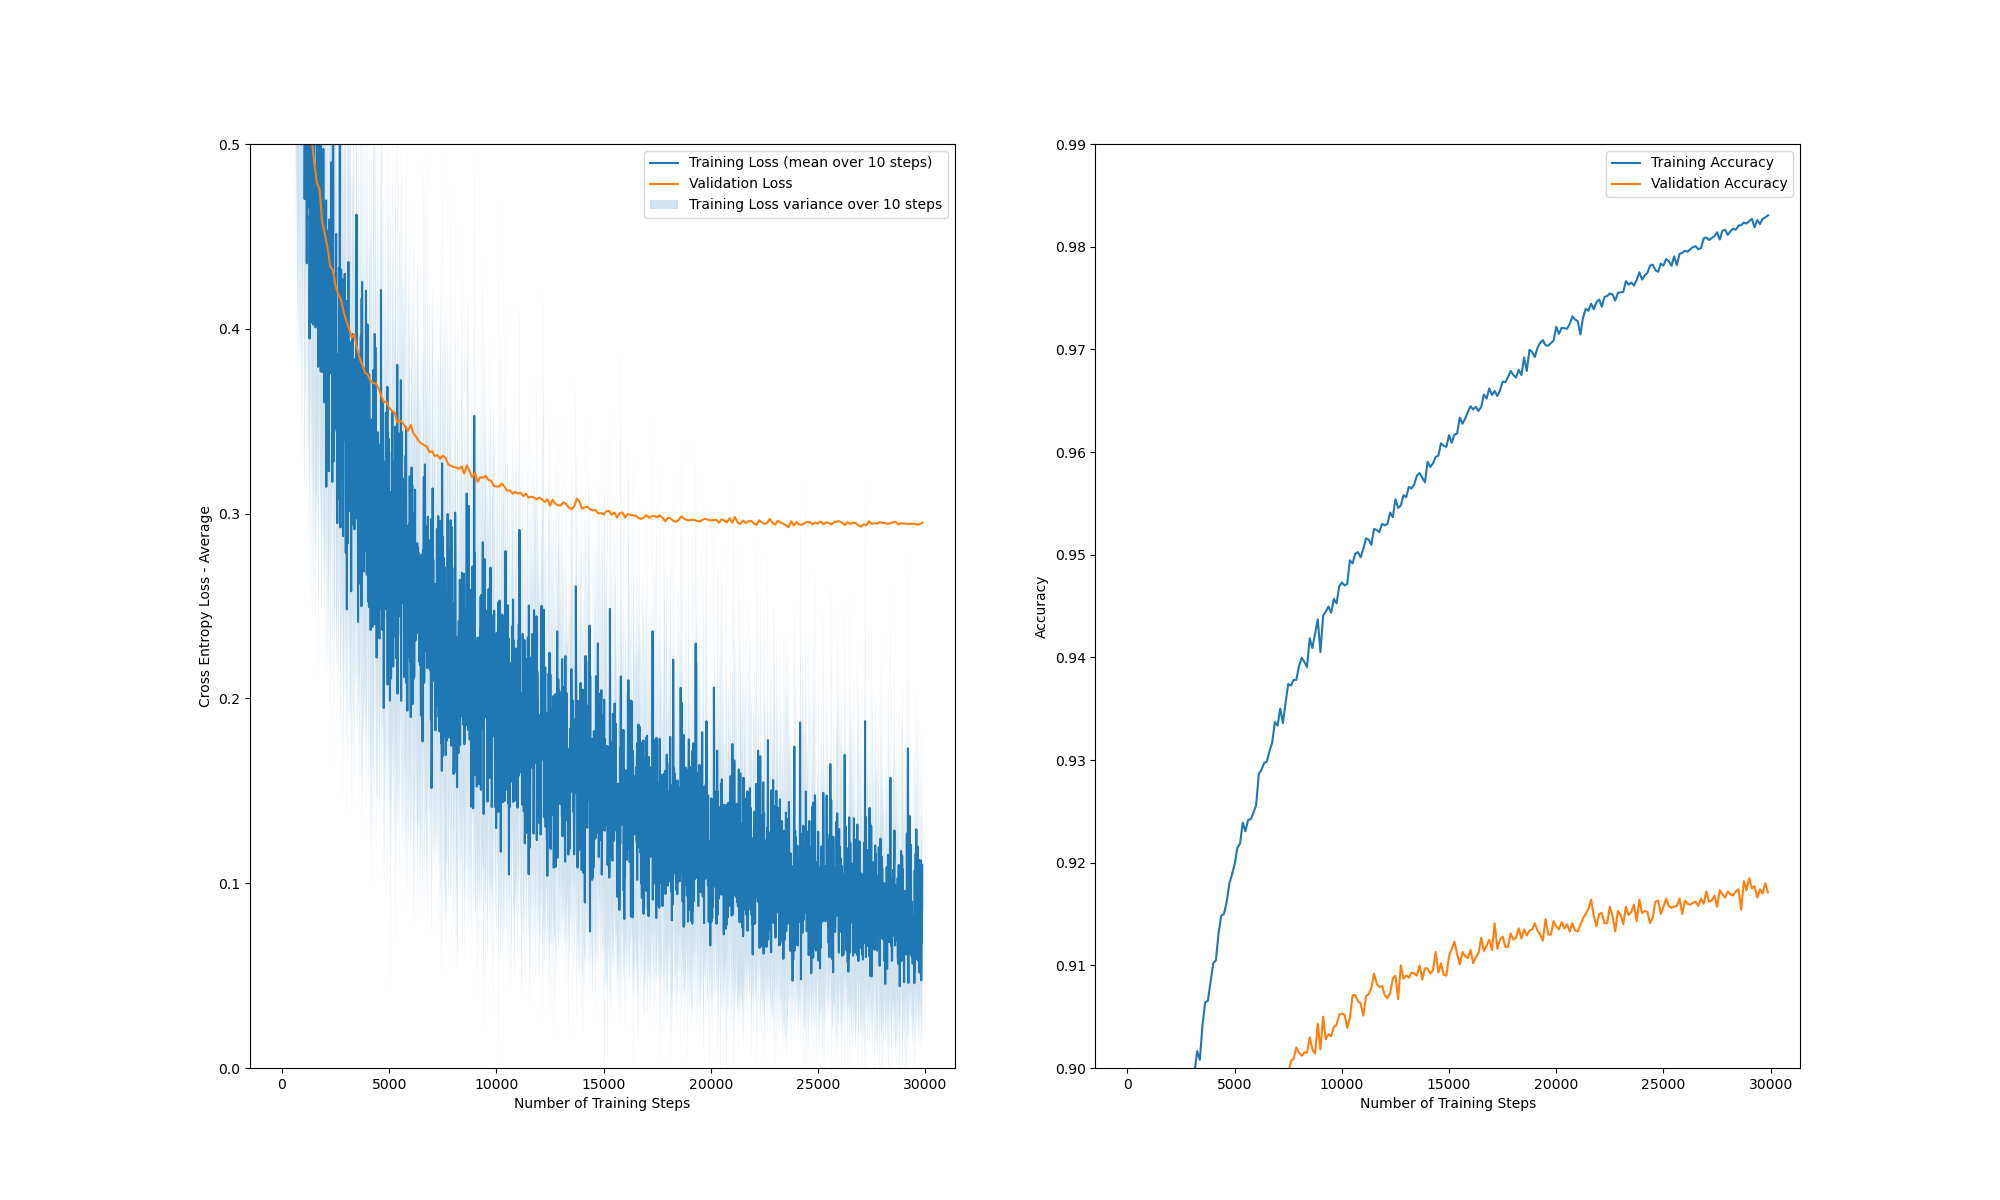
\includegraphics[width=\textwidth]{Assignments/Assignment_2/plots/task2abc/task2c_train_loss.png}
    \caption{Performance of a neural network with two layers. Loss for the training and validation on the left, accuracy for the training and validation set on the right.}
    \label{fig:task2}
\end{figure}


\subsection{Task 2d: Number of parameters}
The number of parameters in the network is defined as the number of weights plus the number of biases. In our case the network has two layers with 64 nodes in the hidden layer and 10 nodes in the output layer. The input vector $\boldsymbol{x}$ consists of 785 elements, 784 data points and 1 bias. This results in two weight matrices, $\mathbf{W_1}$ and $\mathbf{W_2}$, that both have dimensions $[785\times64]$ and $[64\times10]$. The weights include biases, because we have used the bias trick. The resulting number of parameters $P$ is thus:
\begin{equation}
    P = 785\cdot64 + 64\cdot 10 = 50,880 
\end{equation}


\section{Adding the ”Tricks of the Trade”}
In order to improve the performance of the network a few "tricks" has been added to the model. Their impact on the network is shown in \autoref{fig:task3_train} and \autoref{fig:task3_val}. In these plots we see the loss and accuracy for the test and validation set respectively. First the weights in the network were initialized using a normal distribution with mean $\my = 0$ and standard deviation $\sigma = \sqrt{fan-in}$, where $fan-in$ is the number of inputs from the previous layer to the node in the current layer. Secondly a in improved activation function was added in addition to the the normalized weights. This new activation function is zero centered, this helps with giving a large derivative for weights close to zero, thus giving faster convergence. MÅ SKRIVE MER OM DENNE.
Lastly momentum for the gradient descent was added yo the model and the previous improvements. The momentum helps in utilizing a small portion of the previous gradient, this will make the gradient converge faster and may also prevent the network from getting stuck in a local minima as apposed to the desired global minima. 
\begin{figure}[H]
    \centering
    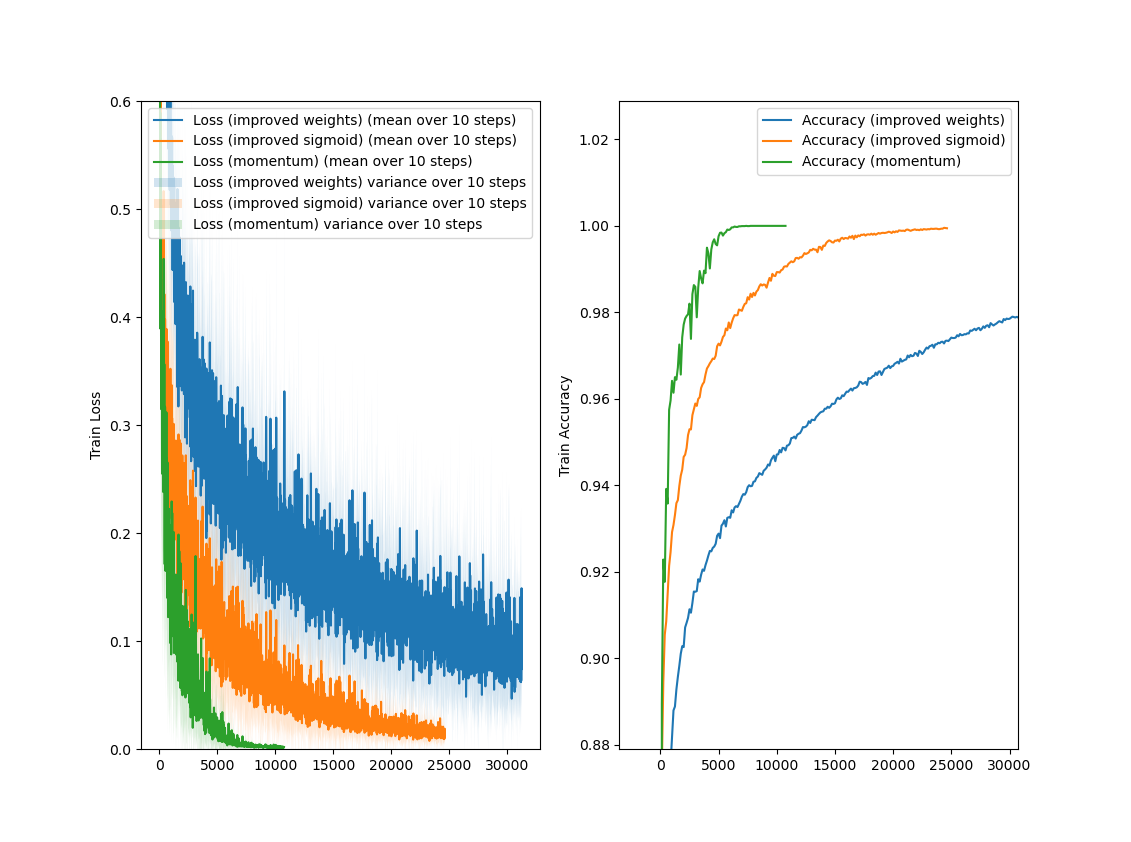
\includegraphics[width=\textwidth]{Assignments/Assignment_2/plots/task3/task3_train.png}
    \caption{Improvements for the network on the training set by adding "Tricks of the Trade".}
    \label{fig:task3_train}
\end{figure}


\begin{figure}[H]
    \centering
    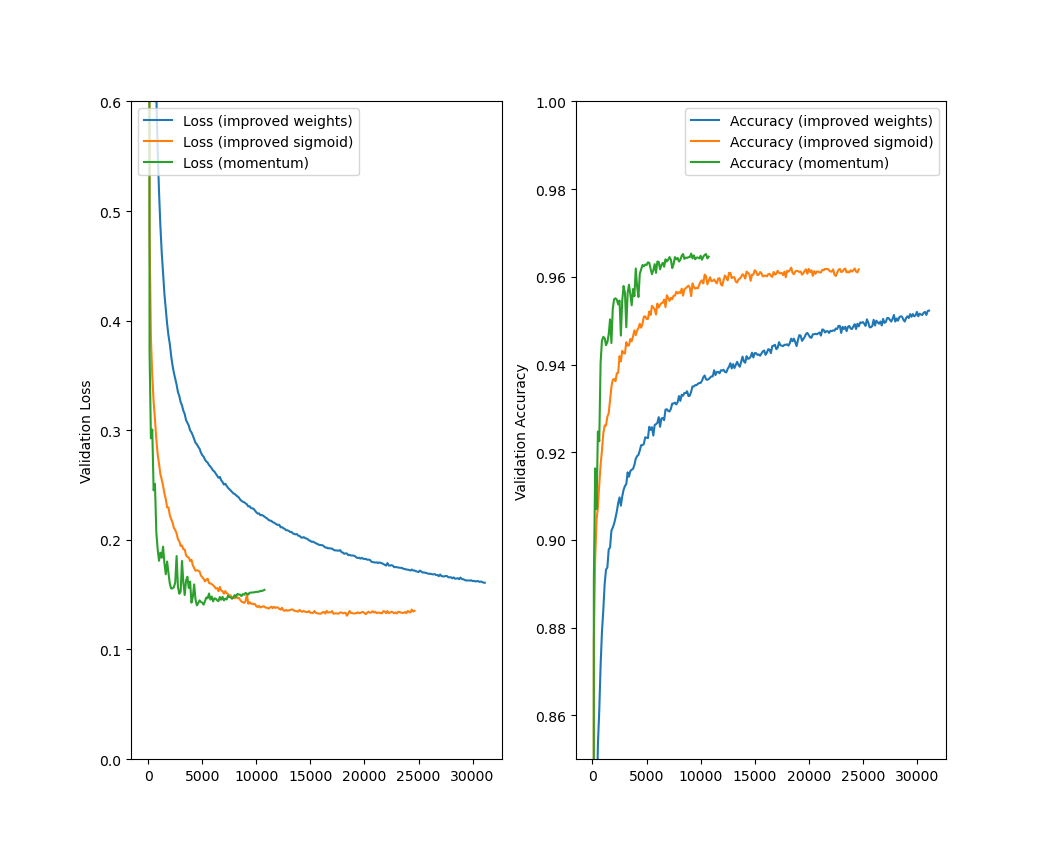
\includegraphics[width=\textwidth]{Assignments/Assignment_2/plots/task3/task3_validation.png}
    \caption{Improvements for the network on the validation set by adding "Tricks of the Trade"}
    \label{fig:task3_val}
\end{figure}

From the plots we see that the network improves both in accuracy and loss for both the training set and the validation set. We see that the network converges significantly faster with each "trick" added. However we see that the network begins to overfit on the training data. We see that the accuracy for training set with momentum is 1, and the validation loss starts to increase at one point. However, the validation accuracy is still improving. NOE SMART HER SOM SIKKRER 8 POINTS 

\section{Experiment with network topology}

\subsection{Task 4ab: Comparison of number of hidden nodes}

In \autoref{fig:4ab-train} and \autoref{fig:4ab-val} we have the loss and accuracy for the training and test sets for different a varying number of hidden nodes. In the comparison we have used the same number of hidden nodes as in the previous tasks, 64 hidden nodes, as a baseline when comparing against an increased size of 128 and a decreased size of 32. 
\begin{figure}[H]
    \centering
    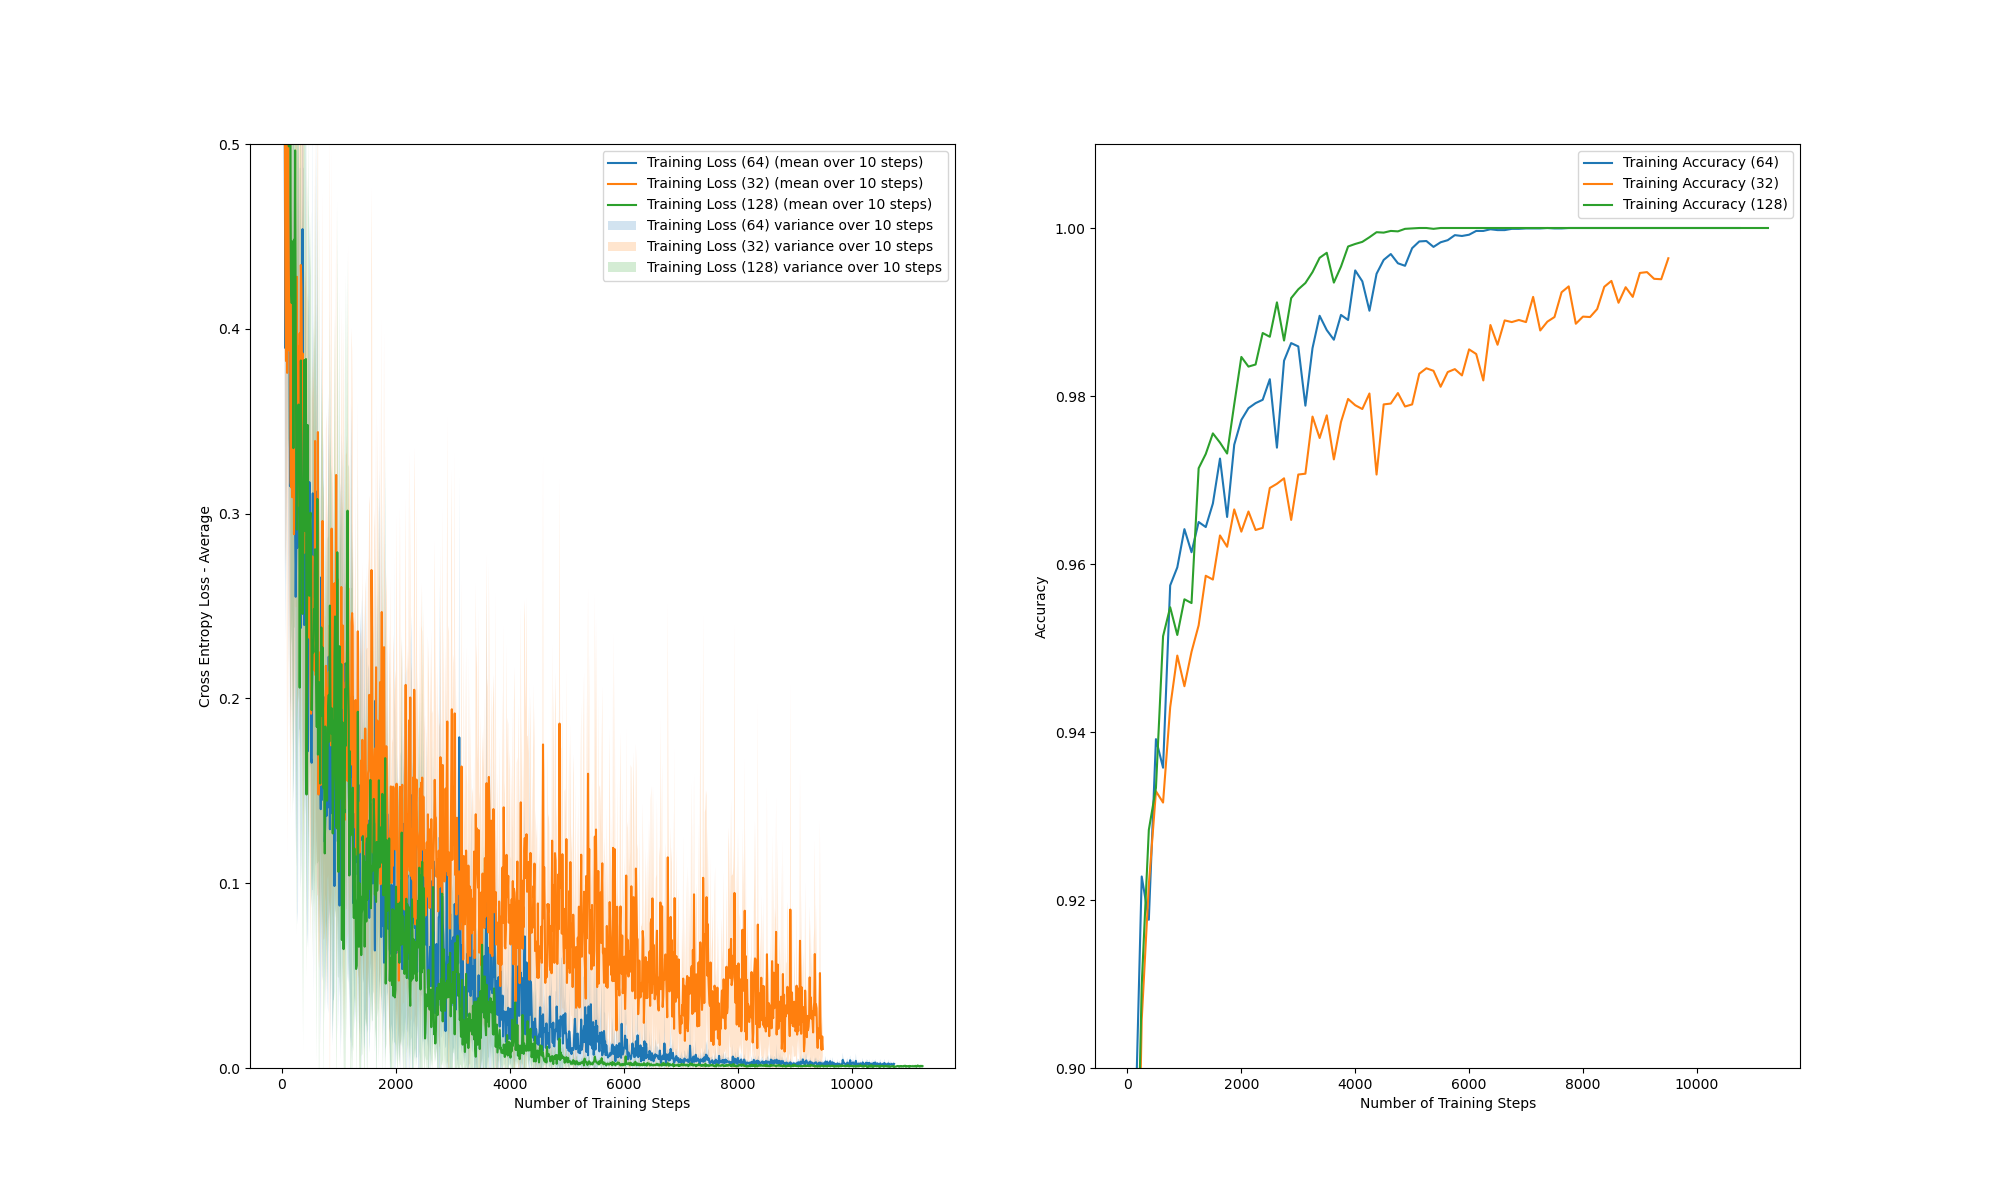
\includegraphics[width=\textwidth]{Assignments/Assignment_2/plots/task4/task4ab_train.png}
    \caption{Comparison of performance impact on the training set with different number of hidden nodes.}
    \label{fig:4ab-train}
\end{figure}

\begin{figure}[H]
    \centering
    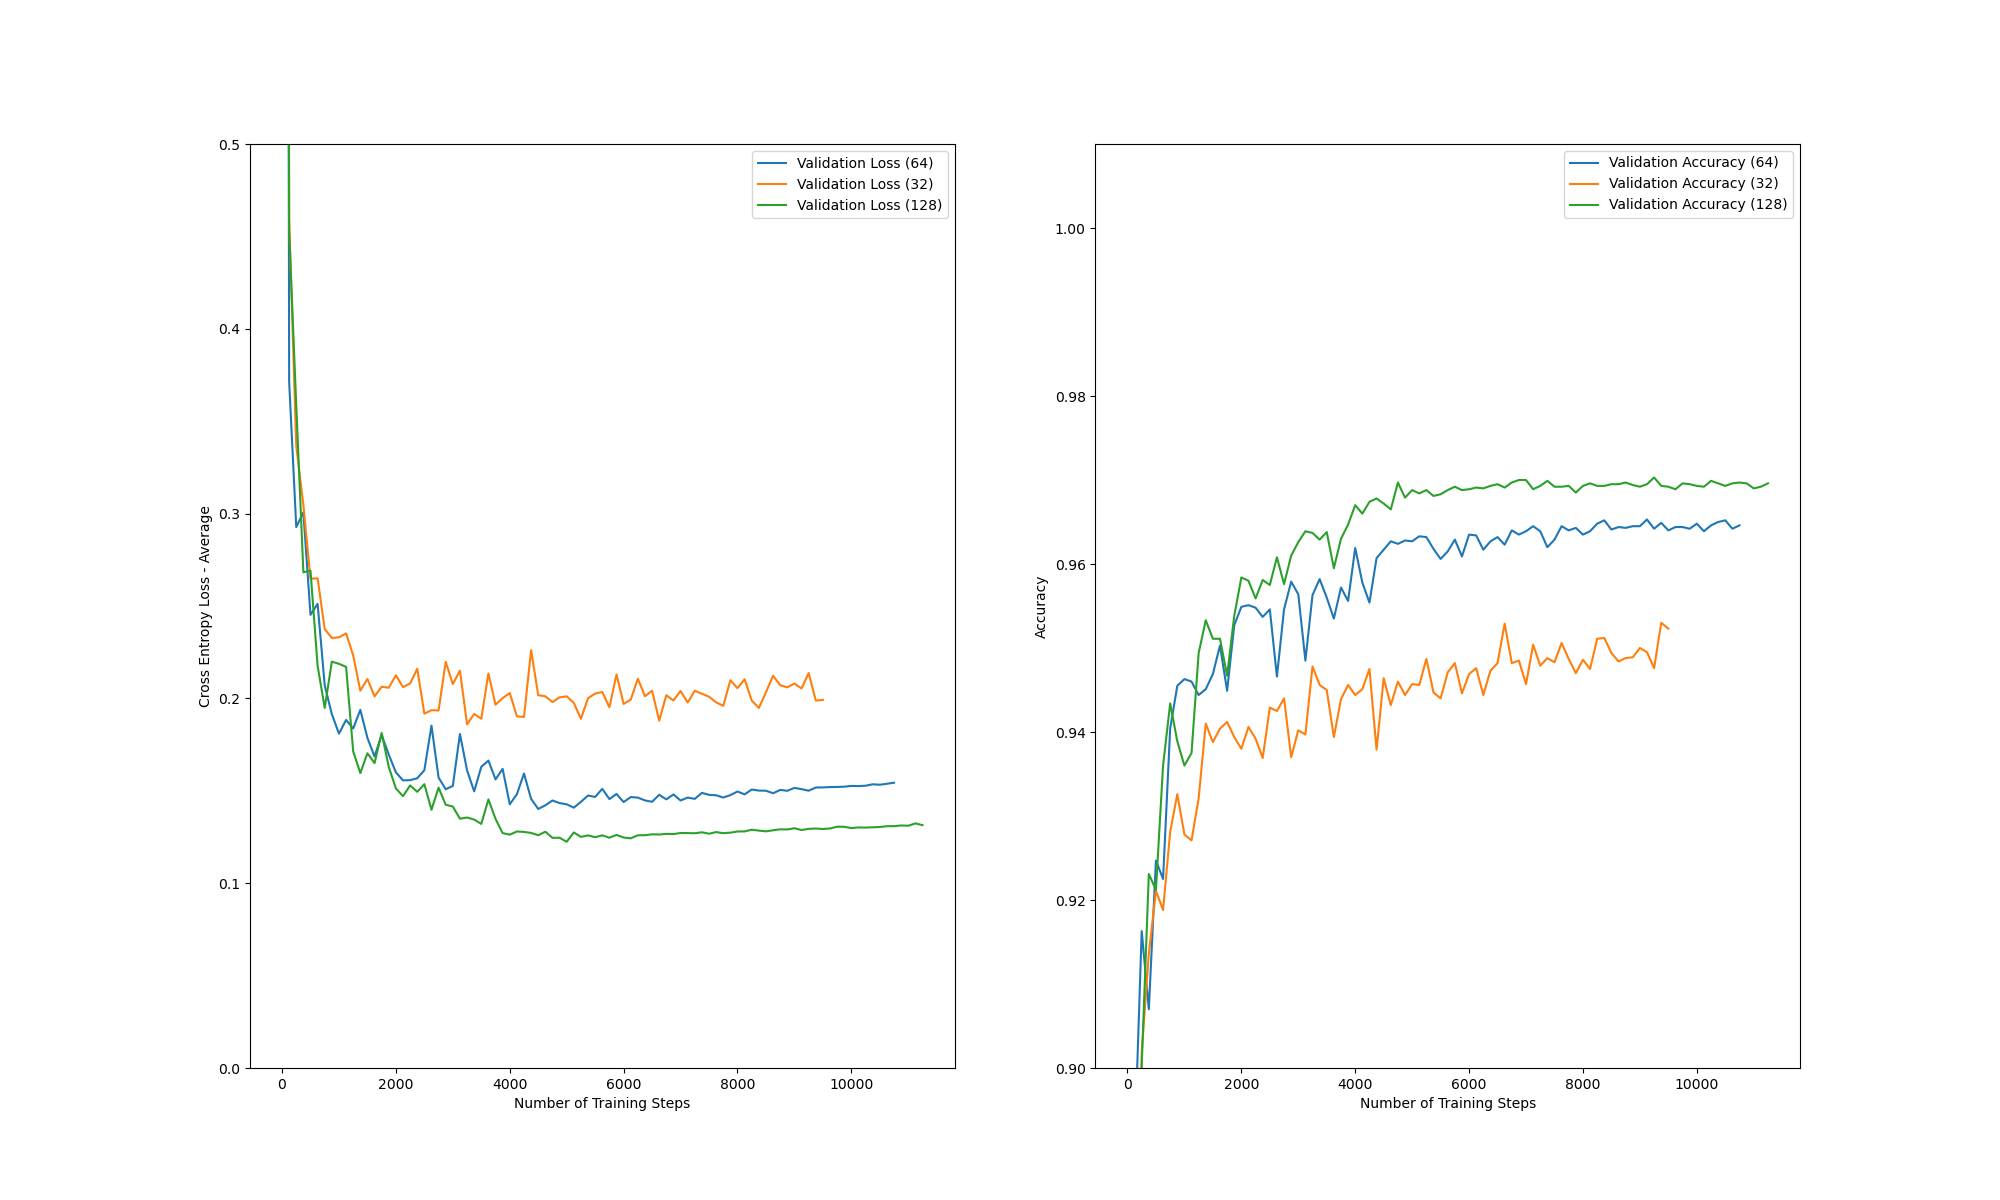
\includegraphics[width=\textwidth]{Assignments/Assignment_2/plots/task4/task4ab_val.png}
    \caption{Comparison of performance impact on the validation set with different number of hidden nodes.}
    \label{fig:4ab-val}
\end{figure}

From the plots we see an increase in performance when adding more hidden units to the model. 

\subsection{Task 4c}

\subsection{Task 4d}
\subsection{Task 4e}
\end{document}